\chapter{Ergebnisse}\label{Ergebnisse}

\section{Evaluation der Anwendung}\label{Evaluation der Anwendung}
\subsection{Funktionale Anforderungen}
Alle funktionalen Anforderungen aus Abschnitt \ref{s.Beschreibung der Anforderungen} sind im Prototyp der Anwendung in Javascript mit dem node.js-Framework und dem socket.io-Websocket-Server aus Abschnitt \ref{socket.io-Server} und -Client aus Abschnitt \ref{socket.io-Client}) vollständig umgesetzt. Im Screenshot des Hamburger Hafens (Abb. \ref{Hafen Hamburg}) kann man erkennen, dass liegende Schiffe als Kreise dargestellt werden und fahrende Schiffe als Richtungsdreiecke. Wurden Reisedaten zu einem Schiff übermittelt (AIS-Nachricht vom Typ 4), sind maßstabsgetreue Polygone eingezeichnet, deren Farbe den Schiffstyp kennzeichnet.
Ein Popup mit Detailinformationen zum dem Schiff links daneben ist geöffnet. In dieser Zoomstufe ist die Animation bereits aktiv, das heißt für den Betrachter, dass alle angezeigten Richtungsdreiecke sich ihrer tatsächlich Geschwindigkeit angemessen bewegen.

\begin {figure}[H]
\begin{center}
  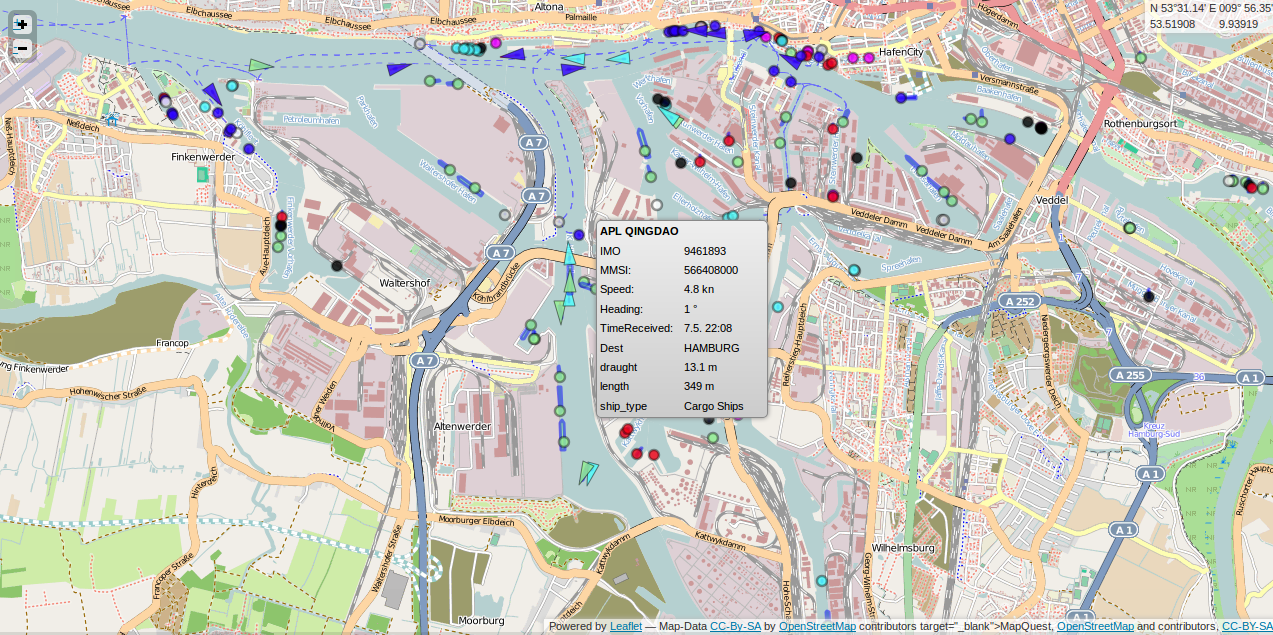
\includegraphics[width=6in]{images/Hamburg.png}
\end{center}
\caption{Anzeige aller Schiffe im Hamburger Hafen}
\label{Hafen Hamburg}
\end {figure}
Abbildung \ref{Nordsee} zeigt die Situation bei niedriger Zoomstufe. Links oben in der Karte ist der Hinweis eingeblendet, dass nur Schiffe mit einer Geschwindigkeit über 12 Knoten angezeigt werden. Die Verteilung des Schiffsverkehrs lässt sich gut erkennen, während die große Zahl hafenliegender Schiffe aus Perfomancegründen ausgespart bleibt. Aus demselben Grund ist die Animation ausgeschaltet. Durch die hohe Frequenz empfangener Positionsmeldungen ist die Darstellung trotzdem in Bewegung.

\begin {figure}[H]
\begin{center}
  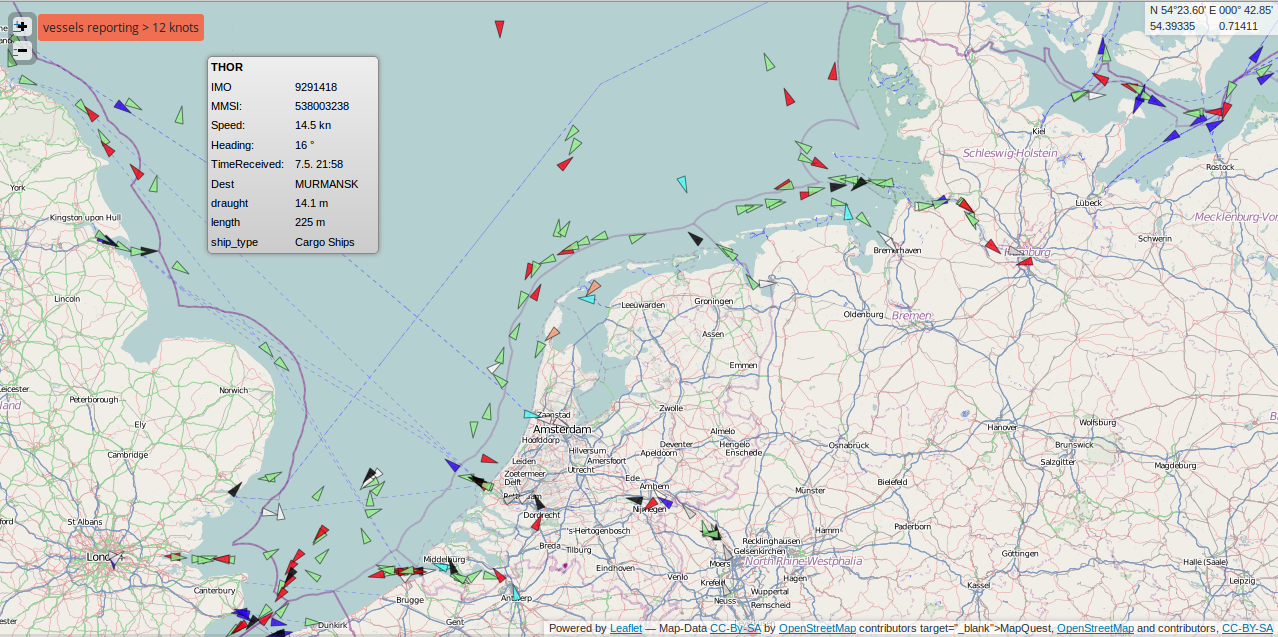
\includegraphics[width=6in]{images/zoomout.png}
\end{center}
\caption{Auf schnell fahrende Schiffe reduzierte Anzeige am Beispiel der Nordsee}
\label{Nordsee}
\end {figure}

\begin {wrapfigure}[9]{r}{3in}
\begin{center}
  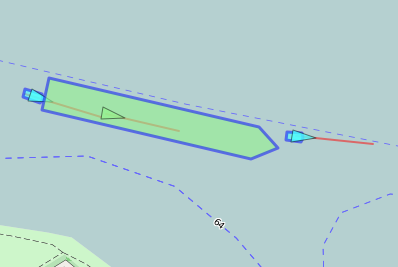
\includegraphics[width=2in]{images/Schleppen.png}
 \caption{Schleppmanöver}
  \end{center}
 \label{Schleppmanöver}

\end {wrapfigure}

Schließlich ist in hohen Zoomstufen eine Beobachtung von aktuellen Schiffsmanövern möglich, wie in Abbildung \ref{Schleppmanöver} das Schleppen eines Frachtschiffes durch zwei Schleppschiffe. Die hohe Frequenz der Positions-Meldungen bei fahrenden Schiffe und die eingebaute Animation lassen den Betrachter die Szene wie in einem Animationsfilm erleben.\\
\subsection{Nicht funktionale Anforderungen}
Die vorgestellte Implementierung erfüllt auch die wichtige nicht funktionale Anforderung nach einer zeitnahen Umsetzung. Sie wurde Ende Februar 2013 an das Unternehmen Vesseltracker übergeben und wird auf github als privates Repository gehostet.
Die gesamte Anwendung ist mit open source Produkten entwickelt worden und verwendet das von der Vesseltracker gehostete OpenstreetMap-Kartenmaterial.\newline
Die Anwendung wurde auf den unten angegebenen Browserclients in den angegebenen Versionen positiv auf Funktionalität getestet und unterstützt damit die gängen Browser in den einschlägigen Versionen \footnote{http://www.browser-statistik.de/statistiken/versionen/}:
\begin{itemize}
\item Firefox Version 15.0.1 und 20.0
\item Google Chrome 26.0
\item Internet Explorer Version 9.0 und 10.0
\item Safari 6.0.4
\end {itemize}

Die Latenzzeit zwischen dem Empfang der AIS-Positions-Meldung durch den Rohdatenserver und der Propagierung derselben Position auf der Karte sollte unterhalb 500 msec liegen. Hier sei verwiesen auf die Ergebnisse in Abschnitt \ref{socket.io- vs html5-Server} und Abbildung \ref{Latenzzeit socket.io}. Die gemessenen Latenzzeiten liegen vollständig innerhalb der geforderten Geschwindigkeit.


Die Anzahl der Verbindungen, die der Server gleichzeitig bedienen kann, ist mit einem node.js-Script getestet worden, das alle 500 ms eine neue Clientverbindung erstellt bis 750 Clients verbunden sind. Der Aufbau der Verbindung geschah auch mit steigender Verbindungsanzahl zuverlässig, jedoch ist in Abbildung \ref{Antwortzeiten socket.io} erkennbar, dass die Anzahl der Fälle zunimmt, in denen ein Client lange auf Antwort warten muss.
\\Eine Skalierung der Serveranwendung ist seitens des socket.io-Servers kein Problem. Statt einen einzigen Worker-Prozess zu generieren, können auch mehrere Worker-Prozesse parallel gestartet werden, die alle dieselbe mongo-Datenbank-Collection abfragen und sich bei derselben redis-Datenbank im Channel ‘positionUpdate’ registrieren können. Allerdings muss sichergestellt sein, z.B.  über unterschiedliche Ports oder unterschiedliche (virtuelle) Server, dass ein verbundener Client mit jedem neuen Request auf demselben Worker-Prozess landet.

\begin{figure}[H]
\begin{minipage}[hbt]{3in}
	\centering
	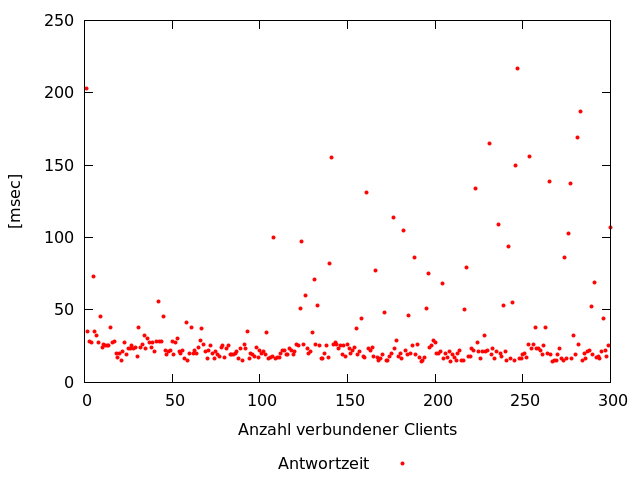
\includegraphics[width=2.5in]{images/stresstest300.png}
	\label{Stresstest300}
\end{minipage}
\hfill
\begin{minipage}[hbt]{3in}
	\centering
	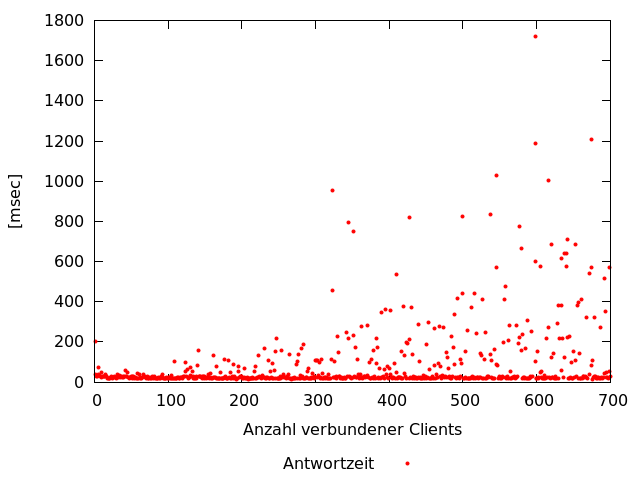
\includegraphics[width=2.5in]{images/stresstest.png}
	\label{Stresstest}
\end{minipage}
\caption{Anwortzeiten des socket.io-Websocket-Servers in Abhängigkeit von der Anzahl verbundener Clients}
\label{Antwortzeiten socket.io}
\end{figure}
%-------------------------------------------------------------------------------------------------------------------------------------------
\section{Vergleichende Evaluation der Javascript- und der Dart-Anwendung}
Für alle folgenden Tests wird auf dem Rohdatenserver ein Port eingerichtet, der nur die Daten von drei AIS-Antennen (Hamburg, Wedel, Geesthacht) als Datenstrom ausgibt. Dies ist notwendig, weil der als Server (und Client) verwendete Arbeitsplatzrechner (HP 530 Notebook PC mit 1,8 GHz Intel Celeron Processor und 1,5 GB Arbeitsspeicher) die Datenmenge aller AIS-Meldungen weltweit nicht in der Geschwindigkeit verarbeiten kann, in der sie eingehen. Dadurch wächst die Messagequeue des Node.js-Servers und erzeugt eine zusätzliche Latenzzeit, die die Ergebnisse verzerrt.

Die in den Abschnitten  \ref{Strategie-Korrektur} und \ref{Vergleichbarkeit} begründete zusätzliche Implementierung eines HTML5-kompatiblen node.js-Websocket-Servers muss nun in einem ersten Schritt mit dem node.js-socket.io-Server verglichen werden. Anschließend wird die in Google Dart geschriebene Client-Anwendung mit dem in Javascript programmierten Client verglichen.
%-------------------------------------------------------------------------------------------------------------------------------------------
\subsection{Vergleich des socket.io-Servers mit dem HTML5-Server}\label{socket.io- vs html5-Server}
\subsubsection{Implementierungsaufwand}
Im Implementierungsaufwand unterscheiden sich beide Server- und Client-Anwendungen kaum. Die Unterschiede in Zeilen Code betragen weniger als 10 Zeilen.\\
Einige Features der socket.io-Bibliotheken (z.B. die Clientverwaltung, Parameter für ‘Production’ und ‘Development’-Umgebung bezüglich Log-Leveln, Client-Minifikation oder Client-Zip) sind praktisch und müssten in der Alternativimplementierung für den Einsatz in einer Produktiv-Umgebung anderweitig gelöst werden. Durch die in socket.io eingeführten Events vermindert sich der Kommunikationsaufwand zwischen Server und Client geringfügig, was in diesem Fall einer datenintensiven Anwendung mit großen Datenmengen pro Nachricht kaum ins Gewicht fällt.
\subsubsection{Latenzzeit}
Die Leistungsfähigkeit beider Implementierungen wird verglichen, indem die Zeit gemessen wird, die eine Positionsmeldung braucht für den Weg vom Rohdatenserver bis zur Präsentation auf der Karte.
Auf dem Rohdatenserver wird jeder AIS-Message beim Empfang ein Zeitstempel (time\_received) hinzugefügt. Dazu läuft auf dem Rohdatenserver ein ntp-Daemon zur Zeitsynchronisation. Genau so ein Daemon läuft auf dem Client, auf dem der Browser gestartet wird. Ein Zeitstempel wird genommen, nachdem das Schiff mit der neuen Position auf die Karte gerendert wurde. Die Latenzzeit berechnet sich dann aus der Differenz zwischen der time\_received und diesem Zeitstempel. \\
Um eine ähnliche Situation in beiden Szenarien abzubilden, wird jeweils eine bestimmte Position im Hamburger Hafen mit maximaler Zoomstufe angesteuert und ein Timer in die Client-Anwendungen integriert, der jeweils nach einer Minute um eine Stufe herauszoomt. Da ab Zoomlevel 11 und kleiner nur noch Schiffe mit einer jeweils definierten Mindestgeschwindigkeit angefordert werden, nimmt die Anzahl empfangener Schiffe von dieser Zoomstufe an wieder ab. Zur Auswertung wird auf dem Client ein LogFile geschrieben, das für jede Positionsmeldung deren ‘time\_received’ und einen aktuellen Zeitstempel festhält. Die Differenz wird als Latenzzeit interpretiert. Anschließend wird über das Logfile berechnet, wieviele Positionsmeldungen in einer Minute an den Client gesendet wurden. In den Abbildungen \ref{Latenzzeit socket.io} und \ref{Latenzzeit HTML5} sind jeweils beide Ergebnisse über die Zeit der Beobachtung (ca. 15 min) aufgetragen.
\begin {figure}[H]
\begin{center}
  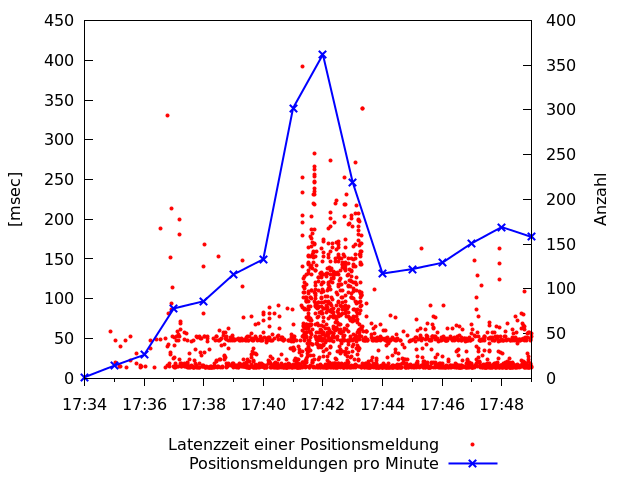
\includegraphics[width=4.5in]{images/latency_timeReceived_socket_io.png}
\end{center}
\caption{socket.io-Websocket-Server: Latenzzeit der Positionsmeldungen und Anzahl empfangener Schiffe}
\label {Latenzzeit socket.io}
\end {figure}

\begin {figure}[H]
\begin{center}
  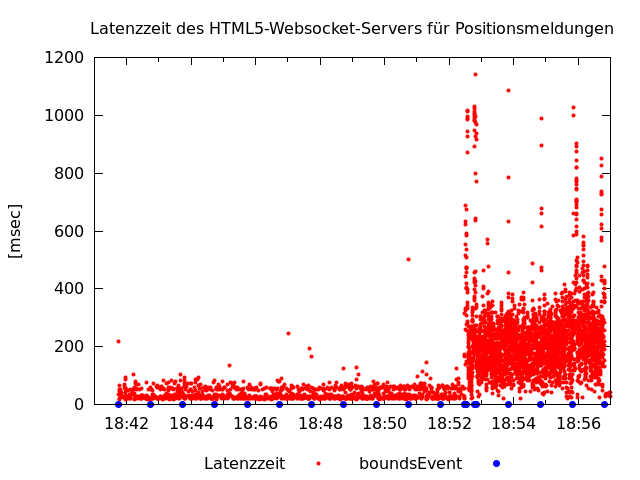
\includegraphics[width=4.5in]{images/latency_timeReceived_HTML5.png}
\end{center}
\caption{HTML5-Websocket-Server: Latenzzeit der Positionsmeldungen und Anzahl empfangener Schiffe}
\label {Latenzzeit HTML5}
\end {figure}
Es ist offensichtlich, dass die Geschwindigkeit in der Darstellung von der Anzahl empfangener Nachrichten linear abhängt.Darüber hinaus ist zu erkennen, dass beide Implementierungen ihre Aufgabe in vergleichbarer Geschwindigkeit erledigen. 
Das bedeutet, dass die HTML5-Node.js-Anwendung in ihrer Leistungsfähigkeit der socket.io-Node.js-Anwendung gleichwertig ist und im Folgenden als repräsentative Javascript-Lösung verwendet werden kann.

\subsubsection{Browserunterstützung}
Für die  node.js-HTML5-Websocket-Anwendung wird wie für die socket.io-Websocket-Anwendung in Abschnitt \ref{Evaluation der Anwendung} die Unterstützung durch die gängigen Browser getestet (Tabelle \ref{Browserclients-Vergleich}).

\begin{table}[H]
\begin{center}
\small
\texttt{
\begin{tabular}{ l|r|c|c}
\bf{Browser}&\bf{Version}&\bf{socket.io}&\bf{HTML5}\\\hline
Firefox& 20.0&websocket&websocket \\
Google Chrome & 26.0 &websocket&websocket\\
Internet Explorer&9& Flashsocket&nicht unterstützt\\
Internet Explorer&10& websocket&websocket\\
Safari&6.0.4 & websocket&websocket\\
\end{tabular}
}
\end{center}
\caption[Unterstützung von Browsern durch die socket.io- und HTML5-Websocket-Clients]{Unterstützung von Browsern durch die socket.io- und HTML5-Websocket-Clients}
\label{Browserclients-Vergleich}
\end{table}

Erwartungsgemäß unterstützen alle gängigen aktuellen Browser HTML5-kompatible Websockets\footnote{http://caniuse.com/\#search=websocket}. Für ältere Browser ohne Websocket-Unterstützung wie den IE 9 bietet socket.io einen Fallback auf Adobe Flashsocket. Listing \ref{flashsocket} zeigt den Client-Request des socket.io-Clients im IE 9, der vom Server den Flashsocket (WebSocketMain.swf) anfordert. In der HTML5-Anwendung dagegen beendet der IE 9  mit einem Scriptfehler die Anwendung.\\
\begin{lstlisting}[language=html,caption=socket.io Client-Request in Internet Explorer 9, label=flashsocket]
Anforderung     GET /socket.io/static/flashsocket/WebSocketMain.swf HTTP/1.1
Accept  */*
Accept-Language de-DE
Referer http://192.168.1.214:8090/ais-socket.io_js.html
x-flash-version 10,0,32,18
Accept-Encoding gzip, deflate
User-Agent      Mozilla/5.0 (compatible; MSIE 9.0; Windows NT 6.1; Trident/5.0)
Host    192.168.1.214:8090                            
\end{lstlisting}

%-----------------------------------------------------------------------------------------------------------------------------------------------
\newpage
\subsection{Vergleich des Javascript-Clients mit dem Dart-Client} 
\subsubsection{Implementierungsaufwand}
Die Möglichkeit des objektorientierten Programmierens in Dart bringt beim Implementieren des Dart-Clients die größte Erleichterung gegenüber der Implementierung in Javascript. Die geschaffene Struktur ist in Abbildung \ref{fig:Übersicht Dart-Files} zu erkennen. Javascript bietet zwar zahlreiche Lösungen, um Objektorientierung nachzubilden, z.B. über Funktionen als Klassen-Objekte und Konstrukte wie das Revealing Module Pattern. Dadurch wird das Programmieren in Javascript aber mit zunehmender Komplexität der Anwendung unübersichtlicher und fehleranfälliger, weil die Features objektorientierter Sprachen sozusagen per Hand gepflegt werden müssen. Die entstehenden Strukturen sind weniger transparent und selbsterklärend als in Dart (\ref{fig:Übersicht Javascript-Files}).
\begin {wraptable}{r}{2in}
\begin{center}
\small
\texttt{
\begin{tabular}{ l|c}
Client&Zeilen Code\\\hline
Javascript& 611 \\
Dart& 867\\
\end{tabular}
}
\caption[Anzahl Zeilen Code im Vergleich der Clients]{Anzahl Zeilen Code im Vergleich der Clients}
\label{Zeilen Code}
\end{center}
\end{wraptable}
Die Dart-Implementierung der Anwendung wird an dem Punkt etwas aufwändiger, wo über das Paket js-interop die Javascript-Dateien integriert werden und Proxies und Callback-Funktionen geschrieben werden müssen zur Kommunikation zwischen dem Javascript- und dem Dart-Kontext. Der quantitative Mehraufwand spiegelt sich auch in einem signifikanten Unterschied in der Anzahl Zeilen Code (Tabelle \ref{Zeilen Code}).\\
Mit dem dart2js-Compiler ließ sich der Dart-Client-Code zu Javascript kompilieren und war dann auch auf Browsern ohne Dart VM ausführbar. Dabei traten gelegentlich Fehler auf, die entweder auf Bugs zurückzuführen waren und mit dem nächsten Update behoben waren oder Fehler, die durch Änderungen im Dart-Code behoben werden mussten, obwohl der originäre Dart-Code von der Dart VM korrekt interpretiert wurde. Dazu ein Beispiel:\\
Wird innerhalb des Javascript-Kontexts eine Methode auf einen Javascript-Proxy (hier \_map) aufgerufen und ein Javascript-Proxy wird zurückgegeben, dann ist es möglich, auf diesen Proxy, der in diesem Fall vom Typ LatLngBounds ist, eine Methode der Klasse LatLngBounds aufzurufen (siehe Listing \ref{LeafletMap.dart}). Im zu Javascript kompilierten Dart-Code lief die Anwendung damit jedoch in einen Fehler:\\
“=> TypeError: t1.get\$\_map(...).getBounds\$0(...).getSouthWest\$0 is not a function”\\

\begin{lstlisting}[caption= LeafletMap.dart mit ursprünglicher Abfrage des Bounds-Objektes, label= LeafletMap.dart]
  List getBounds(){
    var south, west, north, east;
    js.scoped((){
    south= _map.getBounds().getSouthWest().lng;
        west = _map.getBounds().getSouthWest().lat;
        north = _map.getBounds().getNorthEast().lng;
        east = _map.getBounds().getNorthEast().lat;
 });
return [west, south, east, north];
}

 changeRegistration(){
    int zoom = getZoom();
    var boundsList = getBounds();
    Map _southWest = {"lng":boundsList[0],"lat":boundsList[1]};
    Map _northEast= {"lng":boundsList[2],"lat":boundsList[3]};
    Map bounds = {"_southWest": _southWest,"_northEast":_northEast};

    Map message = new Map();
    message['function'] = 'register';
    message['zoom'] =  zoom;
    message['bounds'] = bounds;
    socket.send(stringify(message));
    
    boundsTimeoutTimer = new Timer(new Duration(milliseconds:boundsTimeout),changeRegistration);  
  }
\end{lstlisting}
Weil kein Bug zu diesem Problem über die Dart-Communiy\footnote{https://www.dartlang.org/community/} zu finden ist, wird das Problem mit einem Workaround behoben. Und zwar wird über die Methode ‘getBBoxString’ des Bounds-Objekt ein String mit den Bounds geholt. Aus diesem String sind anschließend die Double-Werte für die Bounds zu parsen (Listing \ref{LeafletMap.dart mit workaround}).
\begin{lstlisting}[caption= LeafletMap.dart mit workaround über BBoxString, label= LeafletMap.dart mit workaround]
String getBounds(){
    String bBox;
    js.scoped((){
      bBox = \_map.getBounds().toBBoxString();
    });
    return bBox;
  }
  changeRegistration(){
    int zoom = getZoom();
    var boundsArray = getBounds().split(",");
    Map _southWest = {"lng":double.parse(boundsArray[0]),"lat":double.parse(boundsArray[1])};
    Map _northEast= {"lng":double.parse(boundsArray[2]),"lat":double.parse(boundsArray[3])};
    Map bounds = {"_southWest": _southWest,"_northEast":_northEast};
    Map message = new Map();
    message['function'] = 'register';
    message['zoom'] =  zoom;
    message['bounds'] = bounds;
    socket.send(stringify(message));
      boundsTimeoutTimer = new Timer(new Duration(milliseconds:boundsTimeout),changeRegistration);  
  }
\end{lstlisting}

\subsubsection{Performance}
Um die Performance des Javascript-Clients mit der des eigentlichen Dart-Clients und des zu Javascript kompilierten Dart-Clients zu vergleichen, wurde der VesselsInBounds-Event genutzt. Gemessen wurde die Zeit, die benötigt wird, um nach Empfang eines VesselInBounds-Events alle in der Message enthaltenen Schiffe auf die Karte zu rendern. Verglichen wurden die Clients in den Browsern Dartium, Chrome und Firefox.
\begin{itemize}
\item Google Dartium interpretiert den originären Dart-Client mit der Dart VM. Beim Aufruf des Javascript-Clients in Dartium wird der Javascript-Code mit der V8-Javascript-Engine interpretiert.
\item Google Chrome  mit der V8-Javascript-Engine führt beim Aufruf des Dart-Clients den zu javascript kompilierten Dart-Code aus und beim Aufruf des Javascript-Clients den originären Javascript-Code.
\item ebenso führt Firefox mit der SpiderMonkey Javascript Engine den zu Javascript kompilierten Dart-Client-Code, bzw. den originären Javascript-Client-Code aus.
\end {itemize}
%\newpage
In einer ersten Testserie wurden die Browserclients auf dem HP 530 Notebook PC mit 1,8 GHz Intel Celeron Processor und 1,5 GB Arbeitsspeicher ausgeführt, auf dem auch die Server-Anwendung läuft.

\begin {figure}[H]
\begin{center}
  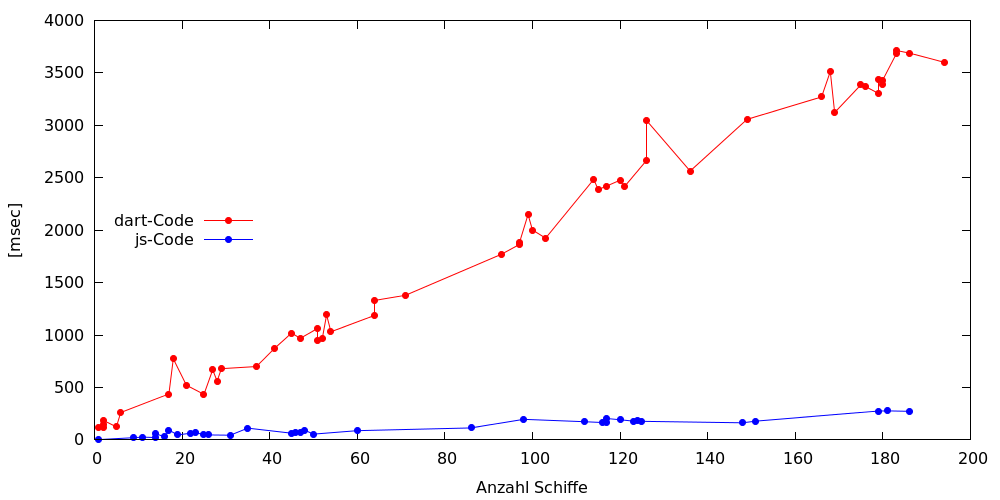
\includegraphics[height=2.3in]{images/Dartium.png}
\end{center}
 \caption{Verarbeitungsdauer in Dartium (HP 530 Notebook PC)}
\end {figure}


\begin {figure}[H]
\begin{center}
  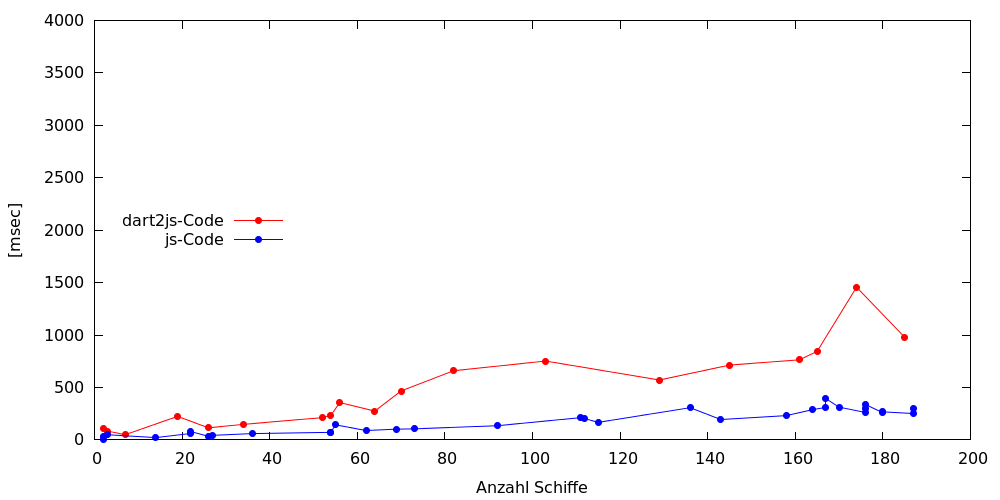
\includegraphics[height=2.3in]{images/Chrome.png}
\end{center}
 \caption{Verarbeitungsdauer in Chrome (HP 530 Notebook PC)}
\end {figure}


\begin {figure}[H]
\begin{center}
  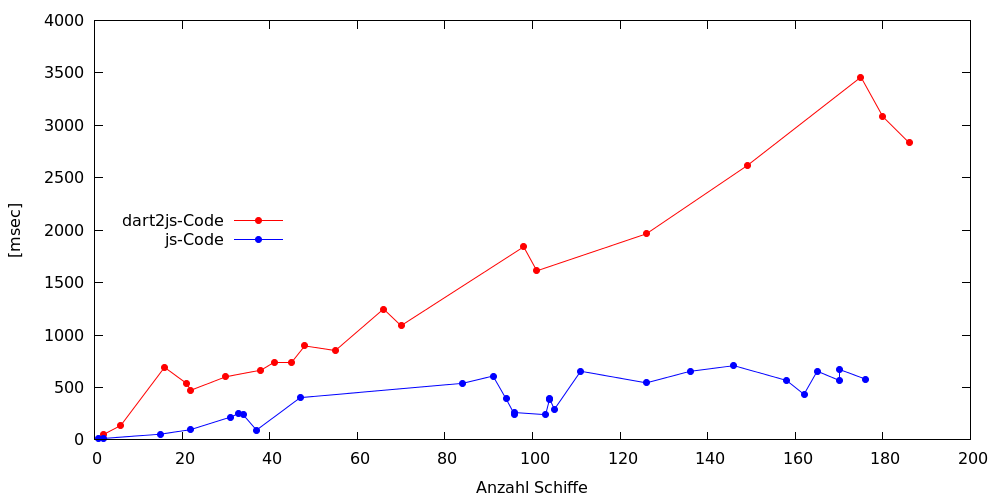
\includegraphics[height=2.3in]{images/Firefox.png}
\end{center}
 \caption{Verarbeitungsdauer in Firefox (HP 530 Notebook PC)}
\end {figure}

%\newpage
In einer zweiten Testserie wurden die Browser-Clients auf einem Apple MacBook Pro 10 mit 2,3 Ghz Intel Core Processor und 8 GB Arbeitsspeicher ausgeführt.
 
\begin {figure}[H]
\begin{center}
  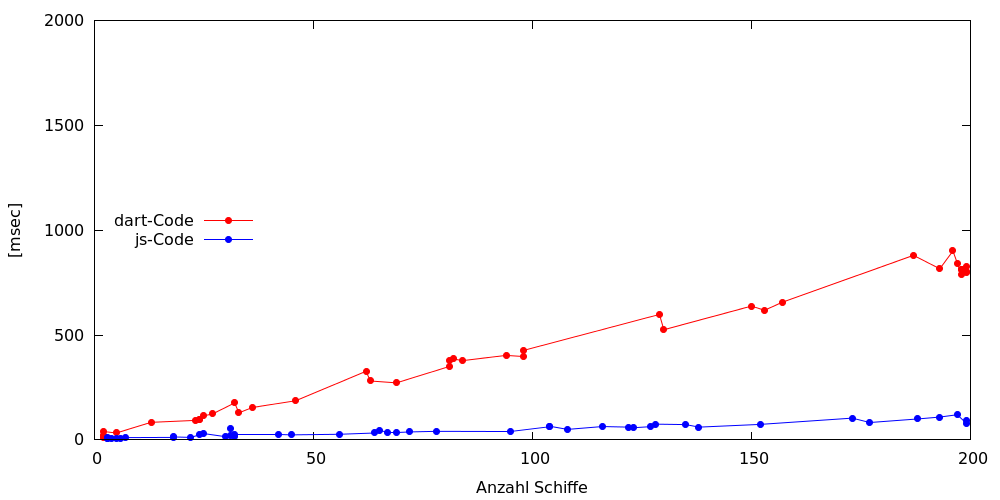
\includegraphics[height=2.3in]{images/DartiumOnMac.png}
\end{center}
 \caption{Verarbeitungsdauer in Dartium (Apple MacBook Pro)}
\end {figure}


\begin {figure}[H]
\begin{center}
  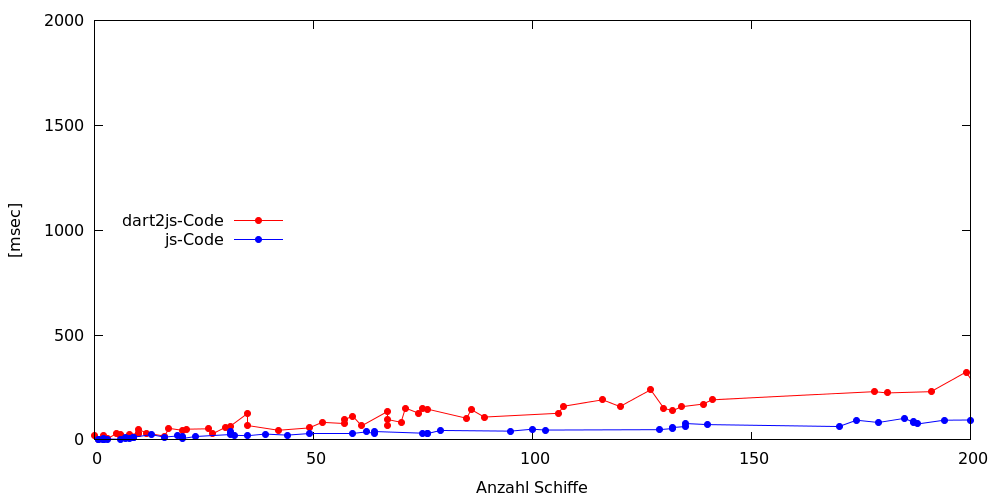
\includegraphics[height=2.3in]{images/ChromeOnMac.png}
\end{center}
 \caption{Verarbeitungsdauer in Chrome (Apple MacBook Pro)}
\end {figure}


\begin {figure}[H]
\begin{center}
  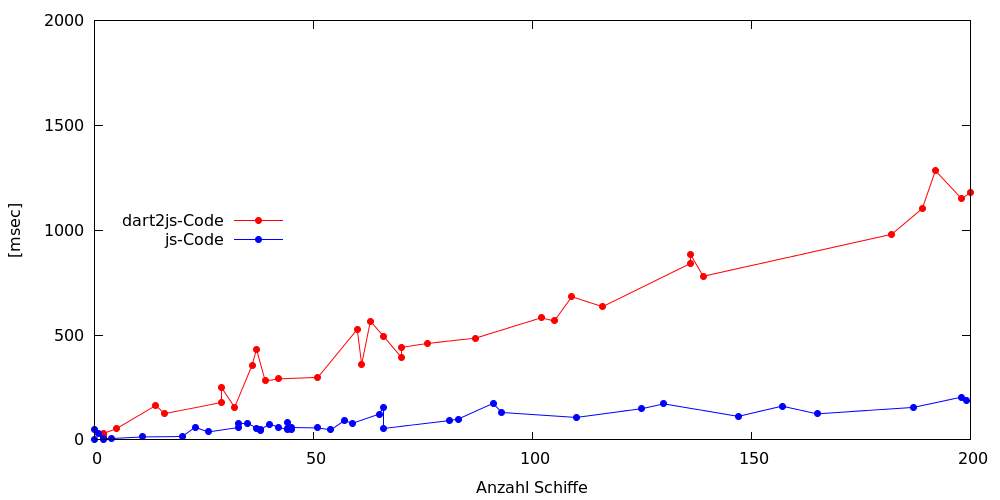
\includegraphics[height=2.3in]{images/FirefoxOnMac.png}
\end{center}
 \caption{Verarbeitungsdauer in Firefox (Apple MacBook Pro)}
\end {figure}

Insgesamt ist erkennbar, dass der Javascript-Code schneller ausgeführt wird als der Dart-Code. Am schnellsten führt die V8-Javascript-Engine in Dartium und Chrome den originären Javascript-Code aus. Firefox mit der Spidermonkey-Javascript-Engine benötigt deutlich länger.\\ Auffällig ist, dass der Dart-Code von der Dart VM in Dartium langsamer ausgeführt wird als der zu Javascript kompilierte Code.
In der zweiten Testserie bestätigen sich diese Ergebnisse. Es ist offensichtlich, dass sich die Geschwindigkeit der Darstellung durch einen leistungsstärkeren Client-Rechner verbessern lässt. Dabei ist deutlich erkennbar, dass der Dart-Client die größte relative Performance-Steigerung erfährt, also am meisten von der zusätzlichen Rechenleistung profitiert.

\subsubsection{Browserunterstützung}
Zusätzlich zu den in den Performance-Tests verwendeten Browsern wurde die Anwendung im InternetExplorer 10 und Safari 6 positiv auf Funktionalität getestet. Das heißt, alle gängigen aktuellen Browser können den zu Javascript kompilierten Dart-Code interpretieren.
%----------------------------------------------------------------------------------------------------------------------------------------------
\chapter{Fazit und Ausblick}\label{Fazit}
%----------------------------------------------------------------------------------------------------------------------------------------------

\section{Die Real-Time-Anwendung}
Der für die Firma Vesseltracker programmierte Prototyp einer Real-Time-Anwendung in Javascript unter Verwendung von node.js mit socket.io ist im Zuge dieser Arbeit Ende Februar 2013 abgeschlossen worden. Die Anwendung soll als zusätzliches Angebot in die Webanwendung der Firma integriert werden. Für einzelne Kunden (z.B. das Maritime Museum Hamburg) ist die Anwendung bereits zugeschnitten und ausgeliefert worden, weitere Kundenprojekte sind geplant.\\

Für die bessere Nutzbarkeit der Anwendung sollte noch eine Möglichkeit geschaffen werden, favorisierte Häfen oder Positionen zu speichern, die per Klick angesteuert werden können, z.B. in einer aufklappbaren Liste.\\
Zur weiteren Optimierung der Anwendung, sollte die Möglichkeit, die Animation der Richtungsdreiecke und Schiffspolygone über css3-Transition-Funktionen zu realisieren, unbedingt weiterverfolgt werden. Damit könnte die vom Browserclient zu erbringende Rechenleistung erheblich reduziert werden, weil die Objekte nicht neu berechnet und erstellt werden müssten, sondern nur über ihre css-Eigenschaften bewegt werden könnten.

%----------------------------------------------------------------------------------------------------------------------------------------------

\section{Vergleich Javascript und Google Dart}
Das Erlernen von Dart ist für Umsteiger von Javascript relativ unkompliziert. Von den vielen Features und Möglichkeiten, die Dart bietet, kommt in der Client-Anwendung nur ein kleiner Teil zum Tragen. Der Fokus lag hier nicht auf den Möglichkeiten von Google Dart, sondern auf der Bewältigung einer konkreten Anforderung. \\
Wie in den Abbildungen zur Struktur der Anwendung erkennbar (Abbildung \ref{fig:Übersicht Dart-Files}), ist mit Dart sehr einfach eine Klassen-Struktur herzustellen. Das macht die Anwendung verständlicher und entsprechend einfacher zu entwerfen, zu schreiben und zu warten.
\\
Hilfreich bei der Entwicklung war der DartEditor als Entwicklungsumgebung. Der Compiler gibt bei Syntax-Fehlern aussagekräftige Fehlermeldungen.\\  
Google Dart befindet sich noch in der Entwicklungsphase, so dass gelegentlich nach den ca. wöchentlichen Versions-Updates von Dart die Anwendung unter der neuen Version nicht mehr lauffähig ist und angepasst werden muss. Belohnt wird dieser Aufwand sozusagen mit einer kontinuierlichen und spürbaren Verbesserung der Performance (Beobachtung im Zeitraum November 2012 bis April 2013).
Das Einbinden existierender Javascript-Bibliotheken mit js-interop erweitert die Nutzungsmöglichen von Dart ganz entscheidend. Das Arbeiten in zwei unterschiedlichen Kontexten (Javascript und Dart) ist am Anfang sehr fehleranfällig. Fehler sind schwierig zu debuggen, weil auch die Debugger (hier Firebug und der Debugger im DartEditor) nur jeweils bis an die Grenzen dieses Kontextes reichen.

Dass in Testserie 2 die Ausführung des Dart-Codes besonders von der besseren Rechenleistung profitiert, lässt vermuten, dass die Kommunikation zwischen den Kontexten innerhalb der Anwendung über Proxies und Callback-Funktionen auch in der Ausführung des Programms einen deutlich höheren Rechenaufwand erzeugt.
Die in dieser Arbeit geschriebene Realtime-Anwendung ist für den ausführenden Client ohnehin sehr rechenintensiv.
\begin{enumerate}
\item werden mit hoher Frequenz Objekte erstellt und gelöscht (besonders durch die Animation der Polygone und Richtungsdreiecke), 
\item werden häufig Events im Dart-Kontext erzeugt (Vessel-Position-Events auf dem Websocket), die Aktionen im Javascript-Kontext notwendig machen und
\item werden bei Benutzeraktionen Events im Javascript-Kontext erzeugt (mouseover-, mouseout- oder moveend-Event), die Aktionen im Dart-Kontext notwendig machen.
\end{enumerate}

Dart bleibt also in der Performance deutlich hinter Javascript zurück. Bei der bisherigen Geschwindigkeit der Entwicklung, insbesondere im Hinblick auf die erlebte Performance-Steigerung, hat Google Dart aber durchaus das Potential, Javascript Konkurrenz zu machen.
Die Einbindung von Javascript-Bibliotheken in Dart ist eine gute Möglichkeit, an die bestehende Web-Welt anzuknüpfen, obwohl der Mehraufwand, der durch die Kommunikation zwischen den beiden Kontexten entsteht sowhl in der Implementierung als auch in der Rechenlast im Browser-Client erheblich ist.\\
Vermutlich wird die Zukunft von Dart sich an zwei Fragen entscheiden:

\begin{itemize}
\item Wie wird die kritische OpenSource Entwicklergemeinde die Sprache aufnehmen, das heißt werden in Zukunft Dart-Bibliotheken in ähnlicher Vielzahl und Diversität entwickelt werden wie in Javascript-Bibliotheken? 
\\
Dr. Axel Rauschmayer beantwortet die Frage, wie quelloffen Google Dart im Vergleich zu Javascript wirklich ist: “
In contrast, Dart is almost proprietary: It is not developed in the open and only shown to the public once it is finished (Brendan Eich calls this ‘delayed-open’). Plus, all of the developers work for Google. It’s great that it is free and eventually open source, both of which will help its popularity. But it probably will never be nearly as open as JavaScript – Google does not have a good track record when it comes to writing specifications for things it open-sources. A recently leaked Android email reminds us that Google is not always as innocent about openness as they sound. Quoting it verbatim:
\begin{itemize}
    \item Do not develop in the open. Instead, make source code available after innovation is complete
    \item Lead device concept: Give early access to the software to partners who build and distribute devices to our specification (ie, Motorola and Verizon). They get a non-contractual time to market advantage and in return they align to our standard.
    \end{itemize}“\cite{google-dart}
\item Wie werden sich die anderen großen Mitspieler auf dem Browsermarkt wie Mozilla, Microsoft und Apple zu Dart positionieren\footnote{http://www.netzwelt.de/news/89916-dart-google-streitet-microsoft-apple-mozilla.html}, das heißt, wird es in Zukunft auch in anderen Browsern Dart Virtual Machines geben?
Dr. Axel Rauschmayer äußert sich dazu: “If you are a competing browser vendor, your prospects for adopting Dart are as follows:
\begin{itemize}
\item    It is difficult to integrate into your existing infrastructure (as you couldn’t give early feedback).
\item    Its development is mainly controlled by Google.
\item    You give Google a head start of over two years.
\end{itemize}
“\cite{google-dart}.
\end{itemize}